% GNUPLOT: LaTeX picture with Postscript
\begingroup
  \makeatletter
  \providecommand\color[2][]{%
    \GenericError{(gnuplot) \space\space\space\@spaces}{%
      Package color not loaded in conjunction with
      terminal option `colourtext'%
    }{See the gnuplot documentation for explanation.%
    }{Either use 'blacktext' in gnuplot or load the package
      color.sty in LaTeX.}%
    \renewcommand\color[2][]{}%
  }%
  \providecommand\includegraphics[2][]{%
    \GenericError{(gnuplot) \space\space\space\@spaces}{%
      Package graphicx or graphics not loaded%
    }{See the gnuplot documentation for explanation.%
    }{The gnuplot epslatex terminal needs graphicx.sty or graphics.sty.}%
    \renewcommand\includegraphics[2][]{}%
  }%
  \providecommand\rotatebox[2]{#2}%
  \@ifundefined{ifGPcolor}{%
    \newif\ifGPcolor
    \GPcolortrue
  }{}%
  \@ifundefined{ifGPblacktext}{%
    \newif\ifGPblacktext
    \GPblacktextfalse
  }{}%
  % define a \g@addto@macro without @ in the name:
  \let\gplgaddtomacro\g@addto@macro
  % define empty templates for all commands taking text:
  \gdef\gplbacktext{}%
  \gdef\gplfronttext{}%
  \makeatother
  \ifGPblacktext
    % no textcolor at all
    \def\colorrgb#1{}%
    \def\colorgray#1{}%
  \else
    % gray or color?
    \ifGPcolor
      \def\colorrgb#1{\color[rgb]{#1}}%
      \def\colorgray#1{\color[gray]{#1}}%
      \expandafter\def\csname LTw\endcsname{\color{white}}%
      \expandafter\def\csname LTb\endcsname{\color{black}}%
      \expandafter\def\csname LTa\endcsname{\color{black}}%
      \expandafter\def\csname LT0\endcsname{\color[rgb]{1,0,0}}%
      \expandafter\def\csname LT1\endcsname{\color[rgb]{0,1,0}}%
      \expandafter\def\csname LT2\endcsname{\color[rgb]{0,0,1}}%
      \expandafter\def\csname LT3\endcsname{\color[rgb]{1,0,1}}%
      \expandafter\def\csname LT4\endcsname{\color[rgb]{0,1,1}}%
      \expandafter\def\csname LT5\endcsname{\color[rgb]{1,1,0}}%
      \expandafter\def\csname LT6\endcsname{\color[rgb]{0,0,0}}%
      \expandafter\def\csname LT7\endcsname{\color[rgb]{1,0.3,0}}%
      \expandafter\def\csname LT8\endcsname{\color[rgb]{0.5,0.5,0.5}}%
    \else
      % gray
      \def\colorrgb#1{\color{black}}%
      \def\colorgray#1{\color[gray]{#1}}%
      \expandafter\def\csname LTw\endcsname{\color{white}}%
      \expandafter\def\csname LTb\endcsname{\color{black}}%
      \expandafter\def\csname LTa\endcsname{\color{black}}%
      \expandafter\def\csname LT0\endcsname{\color{black}}%
      \expandafter\def\csname LT1\endcsname{\color{black}}%
      \expandafter\def\csname LT2\endcsname{\color{black}}%
      \expandafter\def\csname LT3\endcsname{\color{black}}%
      \expandafter\def\csname LT4\endcsname{\color{black}}%
      \expandafter\def\csname LT5\endcsname{\color{black}}%
      \expandafter\def\csname LT6\endcsname{\color{black}}%
      \expandafter\def\csname LT7\endcsname{\color{black}}%
      \expandafter\def\csname LT8\endcsname{\color{black}}%
    \fi
  \fi
    \setlength{\unitlength}{0.0500bp}%
    \ifx\gptboxheight\undefined%
      \newlength{\gptboxheight}%
      \newlength{\gptboxwidth}%
      \newsavebox{\gptboxtext}%
    \fi%
    \setlength{\fboxrule}{0.5pt}%
    \setlength{\fboxsep}{1pt}%
\begin{picture}(7360.00,7080.00)%
    \gplgaddtomacro\gplbacktext{%
      \csname LTb\endcsname%%
      \put(578,5032){\makebox(0,0)[r]{\strut{}\tiny -0.5}}%
      \csname LTb\endcsname%%
      \put(578,5482){\makebox(0,0)[r]{\strut{}\tiny -0.25}}%
      \csname LTb\endcsname%%
      \put(578,5932){\makebox(0,0)[r]{\strut{}\tiny 0}}%
      \csname LTb\endcsname%%
      \put(578,6382){\makebox(0,0)[r]{\strut{}\tiny 0.25}}%
      \csname LTb\endcsname%%
      \put(578,6832){\makebox(0,0)[r]{\strut{}\tiny 0.5}}%
      \csname LTb\endcsname%%
      \put(646,4908){\makebox(0,0){\strut{}\tiny -0.5}}%
      \csname LTb\endcsname%%
      \put(1096,4908){\makebox(0,0){\strut{}\tiny -0.25}}%
      \csname LTb\endcsname%%
      \put(1546,4908){\makebox(0,0){\strut{}\tiny 0}}%
      \csname LTb\endcsname%%
      \put(1995,4908){\makebox(0,0){\strut{}\tiny 0.25}}%
      \csname LTb\endcsname%%
      \put(2445,4908){\makebox(0,0){\strut{}\tiny 0.5}}%
      \colorrgb{1.00,0.00,0.00}%%
      \put(74,5899){\makebox(0,0)[l]{\strut{}O}}%
      \colorrgb{0.00,0.00,1.00}%%
      \put(74,3681){\makebox(0,0)[l]{\strut{}Li}}%
      \colorrgb{0.00,0.32,0.19}%%
      \put(74,1321){\makebox(0,0)[l]{\strut{}Cl}}%
    }%
    \gplgaddtomacro\gplfronttext{%
      \csname LTb\endcsname%%
      \put(1545,7018){\makebox(0,0){\strut{}1 mol/L}}%
    }%
    \gplgaddtomacro\gplbacktext{%
      \csname LTb\endcsname%%
      \put(2847,5032){\makebox(0,0)[r]{\strut{}\tiny -0.5}}%
      \csname LTb\endcsname%%
      \put(2847,5482){\makebox(0,0)[r]{\strut{}\tiny -0.25}}%
      \csname LTb\endcsname%%
      \put(2847,5932){\makebox(0,0)[r]{\strut{}\tiny 0}}%
      \csname LTb\endcsname%%
      \put(2847,6382){\makebox(0,0)[r]{\strut{}\tiny 0.25}}%
      \csname LTb\endcsname%%
      \put(2847,6832){\makebox(0,0)[r]{\strut{}\tiny 0.5}}%
      \csname LTb\endcsname%%
      \put(2915,4908){\makebox(0,0){\strut{}\tiny -0.5}}%
      \csname LTb\endcsname%%
      \put(3365,4908){\makebox(0,0){\strut{}\tiny -0.25}}%
      \csname LTb\endcsname%%
      \put(3815,4908){\makebox(0,0){\strut{}\tiny 0}}%
      \csname LTb\endcsname%%
      \put(4264,4908){\makebox(0,0){\strut{}\tiny 0.25}}%
      \csname LTb\endcsname%%
      \put(4714,4908){\makebox(0,0){\strut{}\tiny 0.5}}%
      \colorrgb{1.00,0.00,0.00}%%
      \put(74,5899){\makebox(0,0)[l]{\strut{}O}}%
      \colorrgb{0.00,0.00,1.00}%%
      \put(74,3681){\makebox(0,0)[l]{\strut{}Li}}%
      \colorrgb{0.00,0.32,0.19}%%
      \put(74,1321){\makebox(0,0)[l]{\strut{}Cl}}%
    }%
    \gplgaddtomacro\gplfronttext{%
      \csname LTb\endcsname%%
      \put(3814,7018){\makebox(0,0){\strut{}10 mol/L}}%
    }%
    \gplgaddtomacro\gplbacktext{%
      \csname LTb\endcsname%%
      \put(5116,5032){\makebox(0,0)[r]{\strut{}\tiny -0.5}}%
      \csname LTb\endcsname%%
      \put(5116,5482){\makebox(0,0)[r]{\strut{}\tiny -0.25}}%
      \csname LTb\endcsname%%
      \put(5116,5932){\makebox(0,0)[r]{\strut{}\tiny 0}}%
      \csname LTb\endcsname%%
      \put(5116,6382){\makebox(0,0)[r]{\strut{}\tiny 0.25}}%
      \csname LTb\endcsname%%
      \put(5116,6832){\makebox(0,0)[r]{\strut{}\tiny 0.5}}%
      \csname LTb\endcsname%%
      \put(5184,4908){\makebox(0,0){\strut{}\tiny -0.5}}%
      \csname LTb\endcsname%%
      \put(5634,4908){\makebox(0,0){\strut{}\tiny -0.25}}%
      \csname LTb\endcsname%%
      \put(6084,4908){\makebox(0,0){\strut{}\tiny 0}}%
      \csname LTb\endcsname%%
      \put(6533,4908){\makebox(0,0){\strut{}\tiny 0.25}}%
      \csname LTb\endcsname%%
      \put(6983,4908){\makebox(0,0){\strut{}\tiny 0.5}}%
      \colorrgb{1.00,0.00,0.00}%%
      \put(74,5899){\makebox(0,0)[l]{\strut{}O}}%
      \colorrgb{0.00,0.00,1.00}%%
      \put(74,3681){\makebox(0,0)[l]{\strut{}Li}}%
      \colorrgb{0.00,0.32,0.19}%%
      \put(74,1321){\makebox(0,0)[l]{\strut{}Cl}}%
    }%
    \gplgaddtomacro\gplfronttext{%
      \csname LTb\endcsname%%
      \put(6083,7018){\makebox(0,0){\strut{}20 mol/L}}%
    }%
    \gplgaddtomacro\gplbacktext{%
      \csname LTb\endcsname%%
      \put(578,2796){\makebox(0,0)[r]{\strut{}\tiny -0.5}}%
      \csname LTb\endcsname%%
      \put(578,3246){\makebox(0,0)[r]{\strut{}\tiny -0.25}}%
      \csname LTb\endcsname%%
      \put(578,3696){\makebox(0,0)[r]{\strut{}\tiny 0}}%
      \csname LTb\endcsname%%
      \put(578,4146){\makebox(0,0)[r]{\strut{}\tiny 0.25}}%
      \csname LTb\endcsname%%
      \put(578,4596){\makebox(0,0)[r]{\strut{}\tiny 0.5}}%
      \csname LTb\endcsname%%
      \put(646,2672){\makebox(0,0){\strut{}\tiny -0.5}}%
      \csname LTb\endcsname%%
      \put(1096,2672){\makebox(0,0){\strut{}\tiny -0.25}}%
      \csname LTb\endcsname%%
      \put(1546,2672){\makebox(0,0){\strut{}\tiny 0}}%
      \csname LTb\endcsname%%
      \put(1995,2672){\makebox(0,0){\strut{}\tiny 0.25}}%
      \csname LTb\endcsname%%
      \put(2445,2672){\makebox(0,0){\strut{}\tiny 0.5}}%
      \colorrgb{1.00,0.00,0.00}%%
      \put(74,5899){\makebox(0,0)[l]{\strut{}O}}%
      \colorrgb{0.00,0.00,1.00}%%
      \put(74,3681){\makebox(0,0)[l]{\strut{}Li}}%
      \colorrgb{0.00,0.32,0.19}%%
      \put(74,1321){\makebox(0,0)[l]{\strut{}Cl}}%
    }%
    \gplgaddtomacro\gplfronttext{%
    }%
    \gplgaddtomacro\gplbacktext{%
      \csname LTb\endcsname%%
      \put(2847,2796){\makebox(0,0)[r]{\strut{}\tiny -0.5}}%
      \csname LTb\endcsname%%
      \put(2847,3246){\makebox(0,0)[r]{\strut{}\tiny -0.25}}%
      \csname LTb\endcsname%%
      \put(2847,3696){\makebox(0,0)[r]{\strut{}\tiny 0}}%
      \csname LTb\endcsname%%
      \put(2847,4146){\makebox(0,0)[r]{\strut{}\tiny 0.25}}%
      \csname LTb\endcsname%%
      \put(2847,4596){\makebox(0,0)[r]{\strut{}\tiny 0.5}}%
      \csname LTb\endcsname%%
      \put(2915,2672){\makebox(0,0){\strut{}\tiny -0.5}}%
      \csname LTb\endcsname%%
      \put(3365,2672){\makebox(0,0){\strut{}\tiny -0.25}}%
      \csname LTb\endcsname%%
      \put(3815,2672){\makebox(0,0){\strut{}\tiny 0}}%
      \csname LTb\endcsname%%
      \put(4264,2672){\makebox(0,0){\strut{}\tiny 0.25}}%
      \csname LTb\endcsname%%
      \put(4714,2672){\makebox(0,0){\strut{}\tiny 0.5}}%
      \colorrgb{1.00,0.00,0.00}%%
      \put(74,5899){\makebox(0,0)[l]{\strut{}O}}%
      \colorrgb{0.00,0.00,1.00}%%
      \put(74,3681){\makebox(0,0)[l]{\strut{}Li}}%
      \colorrgb{0.00,0.32,0.19}%%
      \put(74,1321){\makebox(0,0)[l]{\strut{}Cl}}%
    }%
    \gplgaddtomacro\gplfronttext{%
    }%
    \gplgaddtomacro\gplbacktext{%
      \csname LTb\endcsname%%
      \put(5116,2796){\makebox(0,0)[r]{\strut{}\tiny -0.5}}%
      \csname LTb\endcsname%%
      \put(5116,3246){\makebox(0,0)[r]{\strut{}\tiny -0.25}}%
      \csname LTb\endcsname%%
      \put(5116,3696){\makebox(0,0)[r]{\strut{}\tiny 0}}%
      \csname LTb\endcsname%%
      \put(5116,4146){\makebox(0,0)[r]{\strut{}\tiny 0.25}}%
      \csname LTb\endcsname%%
      \put(5116,4596){\makebox(0,0)[r]{\strut{}\tiny 0.5}}%
      \csname LTb\endcsname%%
      \put(5184,2672){\makebox(0,0){\strut{}\tiny -0.5}}%
      \csname LTb\endcsname%%
      \put(5634,2672){\makebox(0,0){\strut{}\tiny -0.25}}%
      \csname LTb\endcsname%%
      \put(6084,2672){\makebox(0,0){\strut{}\tiny 0}}%
      \csname LTb\endcsname%%
      \put(6533,2672){\makebox(0,0){\strut{}\tiny 0.25}}%
      \csname LTb\endcsname%%
      \put(6983,2672){\makebox(0,0){\strut{}\tiny 0.5}}%
      \colorrgb{1.00,0.00,0.00}%%
      \put(74,5899){\makebox(0,0)[l]{\strut{}O}}%
      \colorrgb{0.00,0.00,1.00}%%
      \put(74,3681){\makebox(0,0)[l]{\strut{}Li}}%
      \colorrgb{0.00,0.32,0.19}%%
      \put(74,1321){\makebox(0,0)[l]{\strut{}Cl}}%
    }%
    \gplgaddtomacro\gplfronttext{%
    }%
    \gplgaddtomacro\gplbacktext{%
      \csname LTb\endcsname%%
      \put(578,436){\makebox(0,0)[r]{\strut{}\tiny -0.5}}%
      \csname LTb\endcsname%%
      \put(578,886){\makebox(0,0)[r]{\strut{}\tiny -0.25}}%
      \csname LTb\endcsname%%
      \put(578,1336){\makebox(0,0)[r]{\strut{}\tiny 0}}%
      \csname LTb\endcsname%%
      \put(578,1786){\makebox(0,0)[r]{\strut{}\tiny 0.25}}%
      \csname LTb\endcsname%%
      \put(578,2236){\makebox(0,0)[r]{\strut{}\tiny 0.5}}%
      \csname LTb\endcsname%%
      \put(646,312){\makebox(0,0){\strut{}\tiny -0.5}}%
      \csname LTb\endcsname%%
      \put(1096,312){\makebox(0,0){\strut{}\tiny -0.25}}%
      \csname LTb\endcsname%%
      \put(1546,312){\makebox(0,0){\strut{}\tiny 0}}%
      \csname LTb\endcsname%%
      \put(1995,312){\makebox(0,0){\strut{}\tiny 0.25}}%
      \csname LTb\endcsname%%
      \put(2445,312){\makebox(0,0){\strut{}\tiny 0.5}}%
      \colorrgb{1.00,0.00,0.00}%%
      \put(74,5899){\makebox(0,0)[l]{\strut{}O}}%
      \colorrgb{0.00,0.00,1.00}%%
      \put(74,3681){\makebox(0,0)[l]{\strut{}Li}}%
      \colorrgb{0.00,0.32,0.19}%%
      \put(74,1321){\makebox(0,0)[l]{\strut{}Cl}}%
    }%
    \gplgaddtomacro\gplfronttext{%
    }%
    \gplgaddtomacro\gplbacktext{%
      \csname LTb\endcsname%%
      \put(2847,436){\makebox(0,0)[r]{\strut{}\tiny -0.5}}%
      \csname LTb\endcsname%%
      \put(2847,886){\makebox(0,0)[r]{\strut{}\tiny -0.25}}%
      \csname LTb\endcsname%%
      \put(2847,1336){\makebox(0,0)[r]{\strut{}\tiny 0}}%
      \csname LTb\endcsname%%
      \put(2847,1786){\makebox(0,0)[r]{\strut{}\tiny 0.25}}%
      \csname LTb\endcsname%%
      \put(2847,2236){\makebox(0,0)[r]{\strut{}\tiny 0.5}}%
      \csname LTb\endcsname%%
      \put(2915,312){\makebox(0,0){\strut{}\tiny -0.5}}%
      \csname LTb\endcsname%%
      \put(3365,312){\makebox(0,0){\strut{}\tiny -0.25}}%
      \csname LTb\endcsname%%
      \put(3815,312){\makebox(0,0){\strut{}\tiny 0}}%
      \csname LTb\endcsname%%
      \put(4264,312){\makebox(0,0){\strut{}\tiny 0.25}}%
      \csname LTb\endcsname%%
      \put(4714,312){\makebox(0,0){\strut{}\tiny 0.5}}%
      \colorrgb{1.00,0.00,0.00}%%
      \put(74,5899){\makebox(0,0)[l]{\strut{}O}}%
      \colorrgb{0.00,0.00,1.00}%%
      \put(74,3681){\makebox(0,0)[l]{\strut{}Li}}%
      \colorrgb{0.00,0.32,0.19}%%
      \put(74,1321){\makebox(0,0)[l]{\strut{}Cl}}%
    }%
    \gplgaddtomacro\gplfronttext{%
    }%
    \gplgaddtomacro\gplbacktext{%
      \csname LTb\endcsname%%
      \put(5116,436){\makebox(0,0)[r]{\strut{}\tiny -0.5}}%
      \csname LTb\endcsname%%
      \put(5116,886){\makebox(0,0)[r]{\strut{}\tiny -0.25}}%
      \csname LTb\endcsname%%
      \put(5116,1336){\makebox(0,0)[r]{\strut{}\tiny 0}}%
      \csname LTb\endcsname%%
      \put(5116,1786){\makebox(0,0)[r]{\strut{}\tiny 0.25}}%
      \csname LTb\endcsname%%
      \put(5116,2236){\makebox(0,0)[r]{\strut{}\tiny 0.5}}%
      \csname LTb\endcsname%%
      \put(5184,312){\makebox(0,0){\strut{}\tiny -0.5}}%
      \csname LTb\endcsname%%
      \put(5634,312){\makebox(0,0){\strut{}\tiny -0.25}}%
      \csname LTb\endcsname%%
      \put(6084,312){\makebox(0,0){\strut{}\tiny 0}}%
      \csname LTb\endcsname%%
      \put(6533,312){\makebox(0,0){\strut{}\tiny 0.25}}%
      \csname LTb\endcsname%%
      \put(6983,312){\makebox(0,0){\strut{}\tiny 0.5}}%
      \colorrgb{1.00,0.00,0.00}%%
      \put(74,5899){\makebox(0,0)[l]{\strut{}O}}%
      \colorrgb{0.00,0.00,1.00}%%
      \put(74,3681){\makebox(0,0)[l]{\strut{}Li}}%
      \colorrgb{0.00,0.32,0.19}%%
      \put(74,1321){\makebox(0,0)[l]{\strut{}Cl}}%
    }%
    \gplgaddtomacro\gplfronttext{%
    }%
    \gplbacktext
    \put(0,0){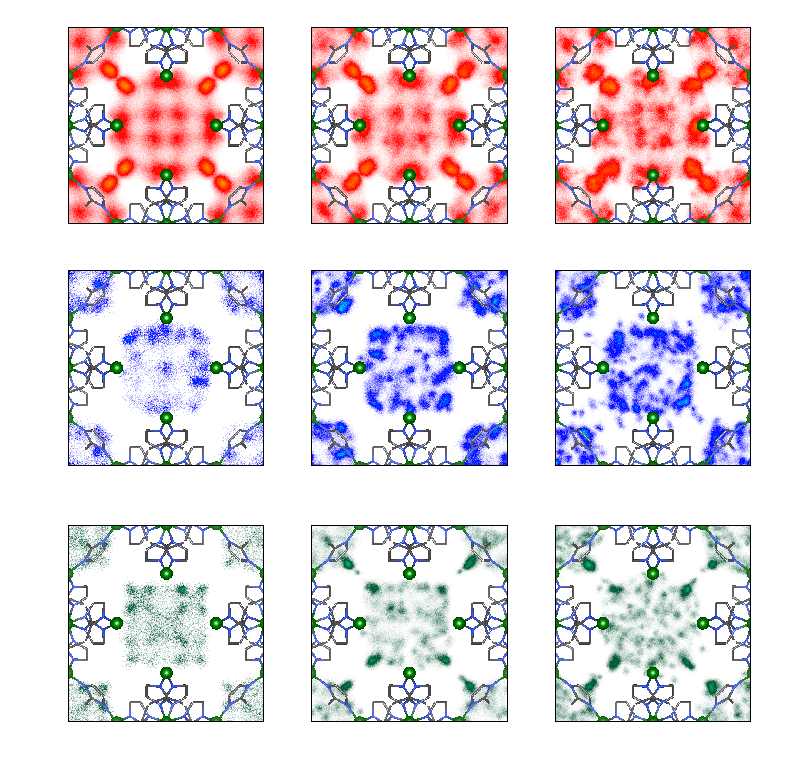
\includegraphics{licl-zif-density}}%
    \gplfronttext
  \end{picture}%
\endgroup
